\section{Design und Architektur}
Beim Design wird auf den Ansatz der Microservices zurückgegriffen, um dessen Vorteile nutzen zu können. Das System ist in seiner Funktionalität stark abhängig von der Verfügbarkeit externer Anwendungen, also dem Jira-System und der Graphdatenbank. Daher ist die Systemarchitektur stark auf die Sicherstellung von Resilienz optimiert. Die Extraktorkomponente soll als verteiltes System implementiert werden, um die Resilienz gegenüber möglichen Ausfällen von Systemkomponenten zu erhöhen. Dabei soll das Extrahieren der Daten und das Laden der Daten in die Zieldatenbank in zwei separaten Services implementiert werden. Die Software soll somit Teilprozesse im ETL-Prozess weiterhin ausführen können auch wenn eine Komponente des Systems nicht verfügbar ist.\\
Für die Kommunikation zwischen den beiden Microservices wird das "Producer-Consumer"-Pradigma eingesetzt.
\subsection{Grundlagen des ETL-Prozesses}
Unsere aufzubauende Datenbank kann als Data-Warehouse betrachtet werden und wird demnach mit Hilfe eines ETL-Prozesses aufgebaut und befüllt. Die Datenbank soll immer bestmöglich den Stand des Quellsystems abbilden. Dies ist durch den Einsatz der periodischen Extraktion zwar nur bedingt möglich, da die Daten nicht in Echtzeit in das Data Warehouse Übertragen werden. Dennoch soll die Periodendauer so kurz gewählt werden, dass die Aktualität der Daten in der Zieldatenbank den Anforderungen ausreichend ist. Eine Möglichkeit der Datenübernahme in den Knowledge Graphen wäre ein periodisch ablaufender Job, welcher alle Änderungen aus dem Quellsystem identifiziert und extrahiert. Wir entscheiden uns aufgrund diverser Vorteile für eine Delta-Extraktion. Es gibt verschiedene Möglichkeiten eine Delta-Extraktion durchzuführen. Unter anderem kann eine Delta-Extraktion durch Trigger, Snapshots oder basierend auf Zeitstempeln durchgeführt werden. Wir entscheiden uns für eine Delta-Extraktion mit Hilfe von Zeitstempeln. Voraussetzung für eine Delta-Extraktion basierend auf Zeitstempeln ist, dass das Quellsystem verlässliche Daten bzw. Zeitstemplen bezüglich Änderungen und dem Anlegen von Objekte verwaltet. Dies muss für alle Objekttypen erfüllt sein, dessen Objekte extrahiert werden sollen [ZITAT Extracting Delta for Incremental Data Warehouse Maintenance]. Dieser Ansatz wird in unserem Fall möglich sein, da ein Jira System für jedes der relevanten Objekttypen standardmäßig ein Feld \glqq Created\grqq\:und \glqq Updated\grqq\:führt, welches uns erlaubt, alle neuen Änderungen im System zu erkennen. \\
Es gilt jedoch zu beachtet, dass ein Zeitstempel, welcher auf eine Änderung eines Objektes hinweist nicht zwangsläufig eine inhaltliche Änderung dieses Objektes bedeutet. Beispielsweise kann ein neuer Kommentar zu einem Ticket hinzugefügt werden. Diese Aktion führt zur Aktualiserung des \glqq Updated\grqq\:-Attributes ohne jedoch das Ticket selbst zu verändern. Daher ist eine weitere Maßnahme notwendig um zu erkennen, ob sich ein Ticket verändert hat. Es wird die Implementierung einer neuen Methode notwendig, welche das Ticket basierend auf dessen Attribute vergleicht und eine Änderung erkennen kann.\\
Der Job lässt sich in zwei Aufgaben unterteilen. Ein Teil davon wird alle neu erstellten Tickets der letzten Periode übernehmen. Der zweite Teil des Jobs wird alle geänderten Tickets der letzten Periode erkennen und die Änderungen extrahieren und übernehmen. Um eine hohe Aktualität des Knowledge Graphen zu gewährleisten ist die Periodendauer möglichst gering zu wählen. \\
Es handelt sich bei diesem ETL-Prozess aufgrund der im Quellsystem vorhandenen Datenstruktur um eine rekursive Delta-Extraktion. Diese Vorgehensweise eignet sich in diesem Fall sehr gut, da die Objekttypen im Quellsystem in einer Baumstruktur vorliegen. Folgende Abbildung verdeutlicht diese Eigenschaft:
% Parallelisierung
Um die Performance der Anwendung zu erhöhen können möglicherweise Extraktionsvorgänge parallel ausgeführt werden. In dieser Arbeit wird die asynchone, parallele Ausführung nicht umgesetzt, da diese weitere Risiken im Zusammenhang mit "Zombie"-Threads oder verwaisten Threads, also Threads die nicht vollendet oder endlos weiterlaufen, birgt. [Zitat]
\subsection{Versionierung}
Das Quellsystem, aus welchem der Knowledge Graph aufgebaut werden soll, befindet sich im operativen Geschäftsumfeld und es muss somit beachtet werden, dass die Daten des Systems nicht konstant sind und regelmäßig Änderungen an den fachlichen Daten des Quellsystems vorgenommen werden können. Im folgenden werden zwei Ansätze betrachtet, um die Versionierung eines Objektes durchzuführen. Basierend auf den Vor- und Nachteilen eines jeden Ansatzes wird eine Vorgehensweise ausgewählt. Eine Möglichkeit besteht darin, die einzelnen Änderungen als Delta zu speichern und [bei Bedarf] aus diesen Änderungen eine Version wiederherzustellen. Der Vorteil dieser Methode liegt im geringen Speicherbedarf. Jedoch wird Rechenleistung benötigt um die Delta-Änderungen auf ein Version zurückzuführen. Ein weiterer Ansatz besteht darin, ganze Kopien eines Objektes anzufertigen und diese zu speichern. In diesem Fall wird mehr Speicherplatz benötigt, aber es muss wenig Rechenleistung aufgewendet werden, um eine Version wiederherzustellen. Im Kern gilt also, dass der benötigte Speicherplatz und Rechenleistung gegeneinander abzuwägen sind. [ZITAT Versioning] \\ 
Die Versionierung muss deterministisch sein um gute Ergebnisse mit der KI zu erzielen. [ZITAT siehe Data Versioning and Its Impact on Machine Learning Models] \\
Die Versionierung in diesem Projekt wird mittels vollständiger Kopien umgesetzt. Die großen Datenmengen welche hierbei entstehen sind tollerierbar, da in Graphdatenbanken keine logischen sondern physische Beziehungen zwischen Objekten führen und wie in [VERWEIS Kapitel 3.3] beschrieben wird immer eine sofortige Referenz auf die neueste Version gewährleistet ist. Um diese Versionierungsstrategie im Knowledge Graphen abzubilden, soll der Zustand eines Objektes zu einem bestimmten Zeitpunkt von seiner Identität entkoppelt werden. Dieses Konzept wird mit dem folgenden Datenbankschema modelliert. Für einzelne Objekttypen kann dieses Schema abweichen und ist somit als Basisschema für alle Objekte zu betrachten, welches je nach Bedarf erweitert werden kann. Bei unserem Konzept ergibt sich eine 1:n-Beziehung der Identität eines Objektes und dessen Zuständen. Verknüpft werden diese beiden Tabellen durch eine Beziehung, welche mindestens das Feld inserted\_at besitzt. Unsere Id-Tabelle hält zudem für jedes Objekt eine Referenz auf dessen aktuellen Zustand. Diese Referenz vereinfacht im Anschluss die Implementierung des Datenzugriff, indem eine Operation mit konstanter Laufzeit den Direktzugriff auf den aktuellen Stand des Objektes erlaubt. Dieses Schema kann wie folgt durch ein ER-Diagram beschrieben werden: [ZITAT einfügen]
\begin{figure}[H]
\centering
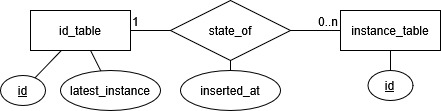
\includegraphics[scale=.6]{dateien/identity_instance_er.jpg}
\caption{Die Identität und Zustände eines Objektes in Form eines ER-Diagramms}
\label{fig:meine-grafik}
\end{figure}
Im Extraktor ist die Implementierung dieses Konzepts nur den jeweiligen Klassen bekannt, welche auf unsere Zieldatenbank zugreifen und diese manipulieren. Durch die Kapselung in den Repository-Klassen bleibt diese Implementierung den Klassen, die fachliche Funtktionen erfüllen verborgen und Datenbankzugriffe können über triviale Methoden stattfinden und vereinfachen somit die Entwicklung erheblich und reduzieren die Fehleranfälligkeit des Codes.
Dass die Datenbank später als Grundlage für einen Chatbot verwendet werden kann, beeinflusst die Art und Weise, wie Objekte in der Graphdatenbank versioniert werden. Ein Vorteil dieses Ansatzes liegt in der unkomplizierten Umsetzung. Es entfällt die Notwendigkeit, Änderungen an einzelnen Feldern zu erkennen und zu versionieren. Außerdem lässt sich der Zustand eines Objektes zu einem Zeitpunkt ohne übermäßigen Aufwand durch eine triviale Datenbankabfrage bestimmten.
Wird in einem zukünftigen Extraktionsvorgang das gleiche Objekt mit einer Änderung seiner Felder erkannt, so wird das Objekt nicht erneut angelegt, sondern lediglich als eine weitere Version dieses Objektes behandelt und in die Tabelle der Instanzen eingefügt.
\subsection{Duplikaterkennung}
Inkonsistenzen können in unserem System entstehen, wenn ein Jira-Ticket fehlerhafte Daten enthält. Existieren zwei Tickets, welche denselben Sachverhalt beschreibt handelt es sich um ein Duplikat. Beschreiben zwei Tickets den gleichen Sachverhalt sind diese nicht als Duplikat zu werten sondern weisen darauf hin, dass ein Problem möglicherweise öfters auftritt und somit schwerwiegender sein könnte. Wahre Duplikate können zu einem Ticket zusammengeführt werden. Zwei Tickets, die mit einer gewissen Wahrscheinlichkeit den gleichen Sachverhalt beschreiben können entweder bei der Übernehme in das Data Warehouse mit einem Ähnlichkeitswert versehen werden oder ohne Ähnlichkeitswert übernommen werden. Im zweiten Fall werden ähnliche oder gleiche Sachverhalten später durch den Chatbot bei Anfragen erkannt. In dieser Arbeit soll die Bestimmung eines Ähnlichkeitswertes bei der Extraktion von Daten aus dem Quellsystem geschehen. Diese Bestimmung kann mittels Künstlicher Intelligenz erfolgen oder durch eigene Applikationslogik implementiert werden. Zum anderen muss beim Design der Ähnlichkeitserkennung die Versionierung betrachtet werden. Um die Komplexität im Hinblick auf die Versionierung zu reduzieren, wird die Ähnlichkeit nur zwischen den Objekten und nicht zwischen den Versionen der Objekte berechnet. In folge dessen wird eine erneute Berechnung der Ähnlichkeiten zu anderen Tickets fällig wenn eine neue Version eines Tickets eingefügt wird. Jede dieser Berechnungen ist aufwändig und es muss ein Konzept entworfen werden um diese Berechnungen effizient durchzuführen. Eine Möglichkeit besteht darin, die Ähnlichkeitswerte nur dann erneut zu brechnen, wenn die neue Version eines Tickets signifikant von der vorherigen Version abweicht. Dazu wird das Ticket mit sich selbst verglichen.\\
Hierbei gibt es verschiedene Herausforderungen zu berücksichtigen. Zum einen muss die Rechenkomplexität beachtet werden, die sich durch das vergleichen von zwei Tickets bei allen Tickets ergibt. Die Rechenkomplexität bezeichnet den Resourcen- und Zeitbedarf einer Rechenoperation mit einer zunehmenden Anzahl n von Objekten. Dieser kann konstant, linear, quadratisch oder exponentiell sein. Im Falle des Vergleichens von Tickets steigt die Rechenkomplexität mit der Anzahl der Tickets quadratisch an [Zitat].\\
Haben sich Informationen im Quellsystem seit der letzten Übernahme geändert, so wird eine neue Version des Tickets angelegt. Eine Änderung lässt sich durch das Feld \glqq Updated\grqq\:bestimmen. Dabei handelt es sich um einen Zeitstempel der letzten Änderung. Welches Feld sich genau geändert hat ist nur durch einen aufwändigeren Abgleich mit der vorherigen Version des Tickets bestimmbar.
\subsection{Resilienz und Fehlertoleranz der Anwendung}
Heuzutage sind nahezu alle Anwendungen auf verschiedene Rechner verteilt und durch Netzwerke miteinander verbunden. Dennoch bleibt die Notwendigkeit bestehen, dass ein verteiltes System sich unverändert zu einem monolithischen System verhält. Jedoch bringen verteilte Systeme Herausforderungen mit sich, welche Maßnahmen im Design erfordern um diese Anforderung erfüllen zu können. Ein zentrales Problem bei verteilten Systemen ist die Netzwerkübertragung und die damit verbundenen möglichen Verzögerungen und Ausfällen. (vgl. van Steen, Pierre und Voulgaris (2012), S. 59-60)